%%%%%%%%%%%%%%%%%%%%%%%%%%%%%%%%%%%%%%%%%%%%%%%%%%%%%%%%%%%%%%%%%%%%%%
% amspaper.tex --  LaTeX-based template for submissions to American 
% Meteorological Society journals
%
% Template developed by Amy Hendrickson, 2013, TeXnology Inc., 
% amyh@texnology.com, http://www.texnology.com
% following earlier work by Brian Papa, American Meteorological Society
%
% Email questions to latex@ametsoc.org.
%
%%%%%%%%%%%%%%%%%%%%%%%%%%%%%%%%%%%%%%%%%%%%%%%%%%%%%%%%%%%%%%%%%%%%%
% PREAMBLE
%%%%%%%%%%%%%%%%%%%%%%%%%%%%%%%%%%%%%%%%%%%%%%%%%%%%%%%%%%%%%%%%%%%%%

%% Start with one of the following:
% DOUBLE-SPACED VERSION FOR SUBMISSION TO THE AMS
\documentclass{ametsoc}

% TWO-COLUMN JOURNAL PAGE LAYOUT---FOR AUTHOR USE ONLY
% \documentclass[twocol]{ametsoc}

%%%%%%%%%%%%%%%%%%%%%%%%%%%%%%%%
%%% To be entered only if twocol option is used

\journal{jamc}

%  Please choose a journal abbreviation to use above from the following list:
% 
%   jamc     (Journal of Applied Meteorology and Climatology)
%   jtech     (Journal of Atmospheric and Oceanic Technology)
%   jhm      (Journal of Hydrometeorology)
%   jpo     (Journal of Physical Oceanography)
%   jas      (Journal of Atmospheric Sciences)	
%   jcli      (Journal of Climate)
%   mwr      (Monthly Weather Review)
%   wcas      (Weather, Climate, and Society)
%   waf       (Weather and Forecasting)
%   bams (Bulletin of the American Meteorological Society)
%   ei    (Earth Interactions)

%%%%%%%%%%%%%%%%%%%%%%%%%%%%%%%%
%Citations should be of the form ``author year''  not ``author, year''
\bibpunct{(}{)}{;}{a}{}{,}

%%%%%%%%%%%%%%%%%%%%%%%%%%%%%%%%

%%% To be entered by author:

%% May use \\ to break lines in title:

\title{Title here}

%%% Enter authors' names, as you see in this example:
%%% Use \correspondingauthor{} and \thanks{Current Affiliation:...}
%%% immediately following the appropriate author.
%%%
%%% Note that the \correspondingauthor{} command is NECESSARY.
%%% The \thanks{} commands are OPTIONAL.

    \authors{Author One\correspondingauthor{Author One, 
     American Meteorological Society, 
     45 Beacon St., Boston, MA 02108.}
 and Author Two\thanks{Current affiliation: American Meteorological Society, 
     45 Beacon St., Boston, MA 02108.}}

     \affiliation{American Meteorological Society, 
     Boston, Massachusetts}

\email{latex@ametsoc.org}


    \extraauthor{Extra Author}
    \extraaffil{Affiliation, City, State/Province, Country}


%%%%%%%%%%%%%%%%%%%%%%%%%%%%%%%%%%%%%%%%%%%%%%%%%%%%%%%%%%%%%%%%%%%%%
% ABSTRACT
%
% Enter your Abstract here

\abstract{Enter the text of your abstract here.  This is a sample American
Meteorological Society (AMS) \LaTeX\ template.  This document provides
authors with instructions on the use of the AMS \LaTeX\ template.  Authors
should refer to the file amspaper.tex to review the actual \LaTeX\ code used
to create this document. The template.tex
file should be modified by authors for their own manuscript.} 

\begin{document}


%% Necessary!
\maketitle


%%%%%%%%%%%%%%%%%%%%%%%%%%%%%%%%%%%%%%%%%%%%%%%%%%%%%%%%%%%%%%%%%%%%%
% MAIN BODY OF PAPER
%%%%%%%%%%%%%%%%%%%%%%%%%%%%%%%%%%%%%%%%%%%%%%%%%%%%%%%%%%%%%%%%%%%%%
%
\section{Introduction}

This document will provide authors with the basic American Meteorological
Society (AMS) formatting guidelines. This document was created using \LaTeX\
and demonstrates how to use the \LaTeX\ template when submitting a manuscript
to the AMS.  The following sections will outline the guidelines and
formatting for text, math, figures, and tables while using \LaTeX\/ for a
submission to the AMS. An attempt to compile amspaper.tex should be made
before using the template. The files have been tested on Windows, Linux, and
Mac OS using \TeX\ Live 2011 (available online at
\url{http://www.tug.org/texlive/}). Feedback and questions should be sent to
latex@ametsoc.org. Additional information is available on the AMS \LaTeX\ Submission Info
web page (\url{http://www2.ametsoc.org/ams/index.cfm/publications/authors/journal-and-bams-authors/author-resources/latex-author-info/}).

Authors should use the empty template.tex to begin their
paper. A valuable source of \LaTeX\ information is the {TeX
Frequently Asked Questions} page (available online at \url{faq.tug.org}).

\section{Formatting text and sections}
The text should be divided into sections, each with a separate heading and
consecutive numbering. Note, however, that single secondary, tertiary, and
quaternary sections remain unnumbered. Each section heading should be placed
on a separate line using the appropriate \LaTeX\ commands. 

\subsection*{Secondary headings} 
Secondary headings labeled with letters are formatted using the
$\backslash$subsection$*${\tt\string{\string}} for a single
subsection within a section or
 or $\backslash$subsection{\tt\string{\string}} 
for multiple
subsections within one section.

\subsubsection*{Tertiary headings} 
Tertiary headings are formatted using the
$\backslash$subsubsection$*${\tt\string{\string}} for single a subsubsection
within a subsection or
$\backslash$subsubsection{\tt\string{\string}} 
for multiple subsubsections
within a subsection. 

\paragraph*{Quaternary headings} 
Quaternary headings are formatted using the
$\backslash$paragraph$*${\tt\string{\string}} for a single paragraph within
a subsubsection or
$\backslash$paragraph{\tt\string{\string}} 
for multiple paragraphs
within a subsection.

\section{Citations}
Citations to standard references in text should consist of the name of the
author and the year of publication, for example, \citet{Becker+Schmitz2003} or
\citep{Becker+Schmitz2003} using the appropriate $\backslash$citet\ or
$\backslash$citep commands, respectively. A variety of citation formats can
be used with the natbib package; however, the AMS prefers that authors use only the $\backslash$citet\ and
$\backslash$citep commands. References should be entered in the references.bib file. For a thorough
discussion of how to enter references into the references.bib database file
following AMS style, please refer to the \textbf{AMS\_Refs.pdf} document
included in this package.

\section{Formatting math}
The following sections will outline the basic formatting rules for
mathematical symbols and units.  In addition, a review of the amspaper.tex
file will show how this is done with the use of \LaTeX\ commands.  The AMS
template provides the American Mathematical Society math, font, symbol, and
boldface packages for use in math mode.

\subsection{Mathematical symbols}
Symbols must be of the same font style both in text discussion and in
displayed equations or terms (and figures should be prepared to match).
Scalar single-character symbols are set italic, Greek, or script. Examples
are $u$, $L$ [note that $\upsilon$ (Greek upsilon) is used instead of
\textit{v} (italic ``vee'') to avoid confusion with $\nu$ (Greek nu) often
used for viscosity; this is handled automatically when in \LaTeX\ math mode],
$w$, $x$, $y$, $z$, $f$, $g$, $r$, indices such as $i$ or $j$, and constants
such as $C_D$, $k$, or $K$. Multiple-character scalar variables,
abbreviations, nondimensional numbers, and acronyms for variables are set
regular nonitalic: $\mathrm{LWC}$, $\mathrm{Re}$, $\mathrm{Ro}$,
$\mathrm{BT}$, $\mathrm{abs}$, $\mathrm{obs}$, $\mathrm{max}$,
$\mathrm{min}$, $\mathrm{Re}$/$\mathrm{Im}$ (real/imaginary), etc. For
vectors, use boldface nonitalic Times Roman as in $\mathbf{V}$, $\mathbf{v}$,
or $\mathbf{x}$, and $\mathbf{i}$, $\mathbf{j}$, and $\mathbf{k}$ unit
vectors. Do not use the \LaTeX\ $\backslash$vec command to denote vectors.
For matrix notation, use nonitalic boldface Arial (or sans serif) font as in
$\pmb{\mathsf{A}}$, $\pmb{\mathsf{B}}$, or $\pmb{\mathsf{M}}$. Note that you will need to use the 
$\backslash$pmb command for boldface sans serif; the $\backslash$bm command will not work. All mathematical
operator abbreviations/acronyms are set lowercase regular Roman font, except
$O$ (on the order of): $\sin$, $\cos$, $\tan$, $\tanh$, $\mathrm{cov}$, $\Pr$
(for probability; note same as Prandtl number), $\mathrm{const}$ (for
constant), $\mathrm{c.c.}$ (complex conjugate).

\subsection{Units}
Units are always set on a single line with a space separating the
denominator, which is set with a superscript $-1$, $-2$, and so on, rather
than using a slash for ``per.'' Examples are g kg$^{-1}$, m$^2$ s$^{-1}$, W
m$^{-2}$, g m$^{-3}$, and m s$^{-1}$ (note that ms$^{-1}$ is the unit for
``per millisecond'').

\subsection{Equations}
Brief equations or terms set inline in text must be set as a single-line
expression because page proofs are not double spaced, for example,
$\rho^{-1}p/x$ or $(1/{\rho})p/x$ or $(a-b)/(c+d)$; that is, use a
superscript $-1$ for the denominator. In case of a more complicated term or
equation, it should be set as an unnumbered display equation, such as
\begin{displaymath} x=\frac{2b\pm\sqrt{b^{2}-4ac}}{2c}.  \end{displaymath}

Otherwise, numbered display equations can be entered using the appropriate
equation command, such as \begin{equation}
x=\frac{2b\pm\sqrt{b^{2}-4ac}}{2c}.  \end{equation}

Lists of equations are punctuated as written English, and commas, semicolons,
and periods are placed where appropriate. Conjunctions such as ``and,''
``while,'' ``when,'' or ``for'' are also typically placed before the final
element in a mathematical phrase, as befits the intended mathematical
meaning.  

\section{Figures and tables}
The AMS prefers that all figures and tables are placed {\bf at the end of the document} prior to submission. 
A list of tables and a list of figures will appear near the end of the PDF
file, before the actual tables and figures. These lists are necessary for submission.

For appendix figures and tables, special commands are needed to manually 
change the numbering to ensure that each appendix figure or table is numbered 
as part of the respective appendix and not as a continuation of the main paper. Use the command
$\backslash$appendcaption\{\} instead of the usual $\backslash$caption\{\} to adjust the 
numbering; for example, for Table A1, you would use the command \verb+\appendcaption{A1}+.

Note that the normal $\backslash$ref\{\} command cannot be used to cite 
appendix figures and tables as the numbering will be incorrect. Callouts for appendix figures 
and tables in the text will need to be written out as plain text, for example, Fig. A1 and Table A1.

\subsection{Figures}
The insertion of a sample figure (Fig. \ref{f1})  
and caption is given below (in the .tex document) and at the end of the document. Standard figure sizes are 19 (one column), 
27, 33, and 39 (two columns) picas.

%%%%%%%%%%%%%%%%%%%%%%%%%%%%%%%%%%%%%%%%%%%%%%%%%%%%%%%%%%%%%%%%%%%%%
% FIGURES---PLACE AT END OF DOCUMENT
%%%%%%%%%%%%%%%%%%%%%%%%%%%%%%%%%%%%%%%%%%%%%%%%%%%%%%%%%%%%%%%%%%%%%
%\begin{figure}[h]
% \centerline{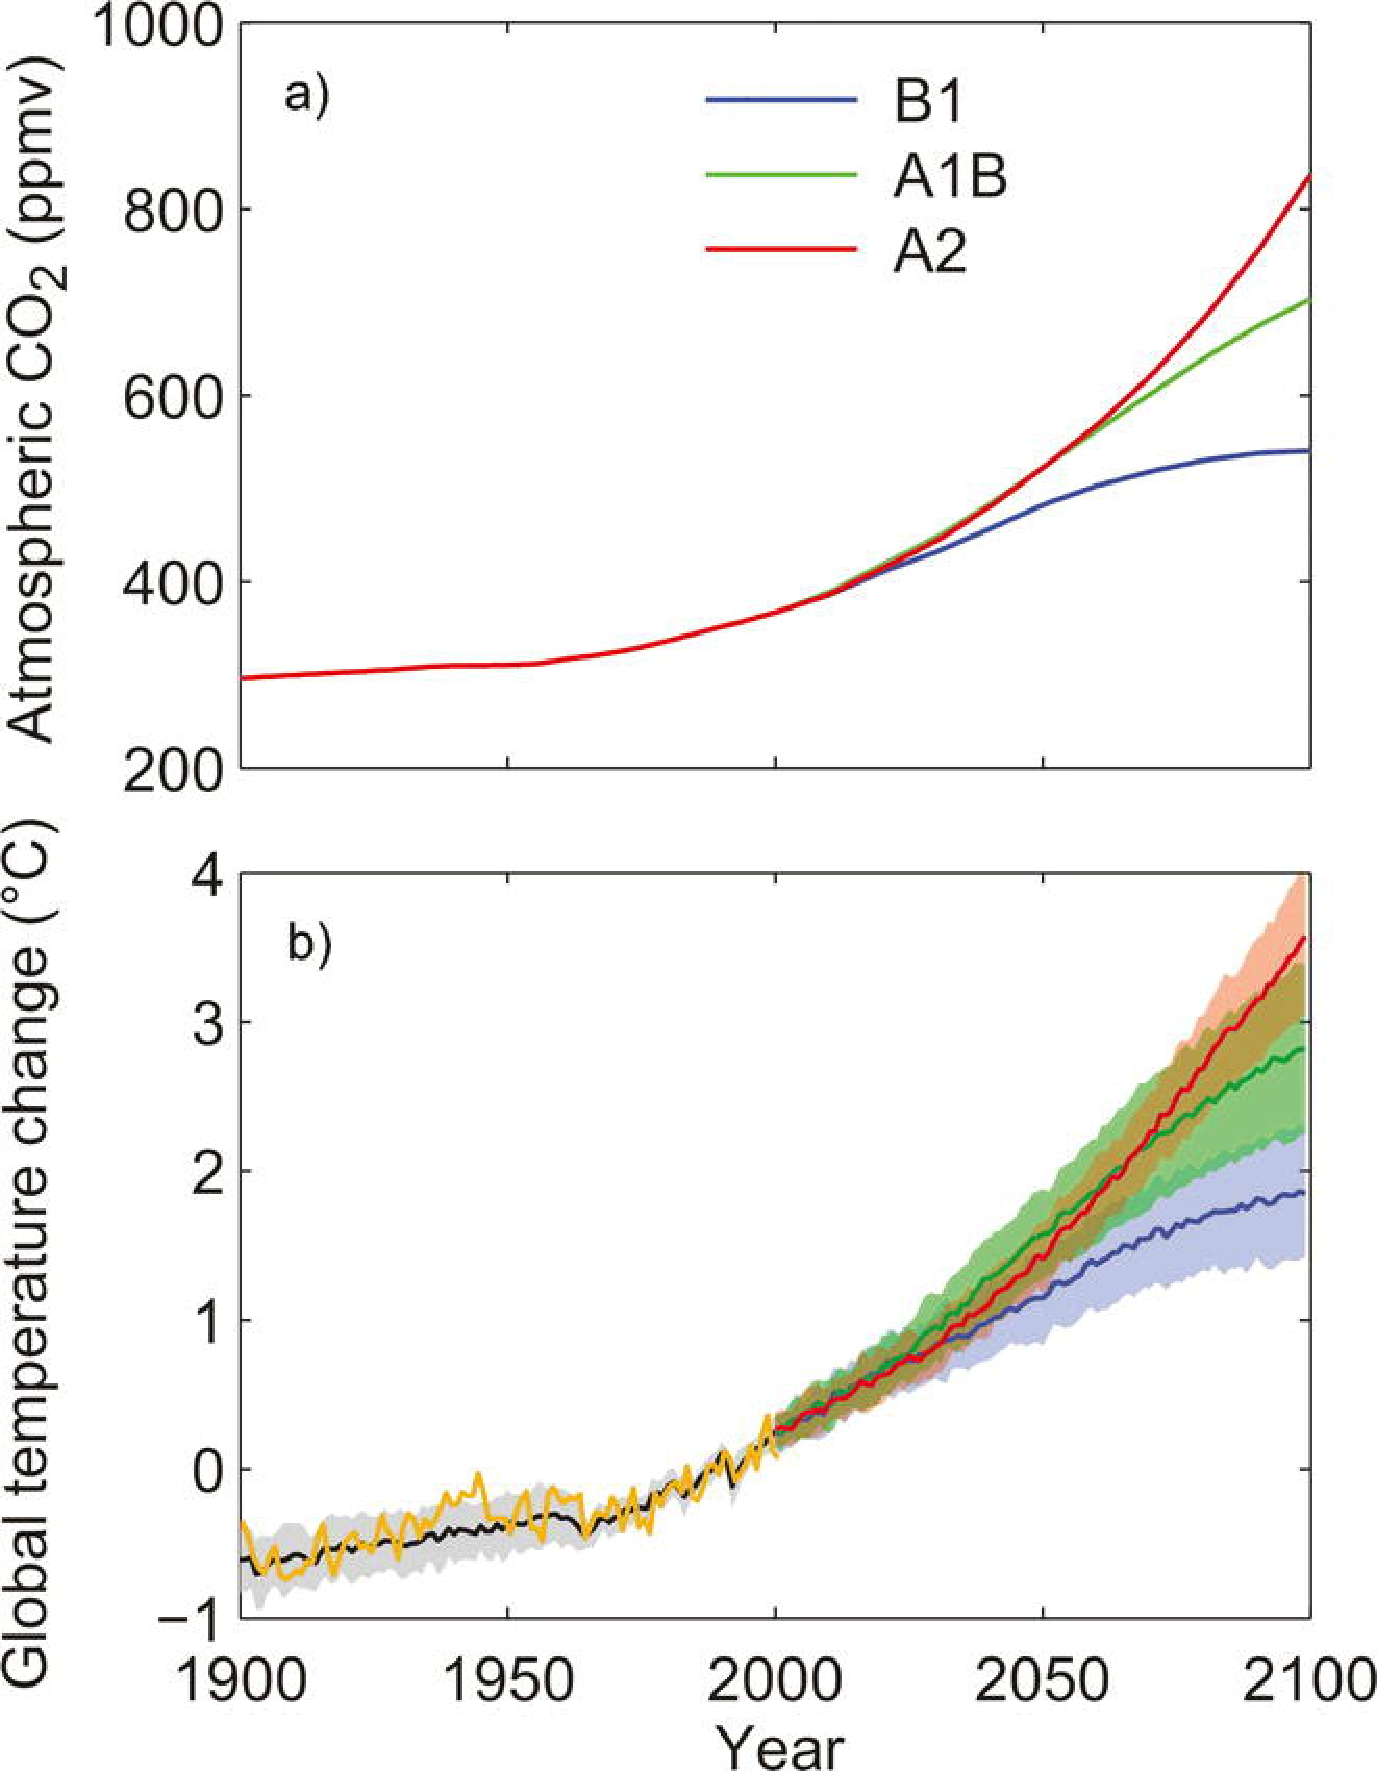
\includegraphics[width=19pc]{figure01.pdf}}
%  \caption{Enter the caption for your figure here.  Repeat as
%  necessary for each of your figures. Figure from \protect\cite{Knutti2008}.}\label{f1}
%\end{figure}
%

\subsection{Tables}
Each table must be numbered, provided with a caption, and mentioned
specifically in the text. 
See below (in the .tex document) and at the end of the document for the formatting of a sample table (Table
\ref{t1}).

%%%%%%%%%%%%%%%%%%%%%%%%%%%%%%%%%%%%%%%%%%%%%%%%%%%%%%%%%%%%%%%%%%%%%
% TABLES---PLACE AT END OF DOCUMENT
%%%%%%%%%%%%%%%%%%%%%%%%%%%%%%%%%%%%%%%%%%%%%%%%%%%%%%%%%%%%%%%%%%%%%
%\begin{table}[h]
%\caption{This is a sample table caption and table layout.  
%Table from Lorenz (1963).}\label{t1}
%\begin{center}
%\begin{tabular}{ccccrrcrc}
%\topline
%$N$ & $X$ & $Y$ & $Z$\\
%\midline
% 0000 & 0000 & 0010 & 0000 \\
% 0005 & 0004 & 0012 & 0000 \\
% 0010 & 0009 & 0020 & 0000 \\
% 0015 & 0016 & 0036 & 0002 \\
% 0020 & 0030 & 0066 & 0007 \\
% 0025 & 0054 & 0115 & 0024 \\
%\botline
%\end{tabular}
%\end{center}
%\end{table}
%%

%%%%%%%%%%%%%%%%%%%%%%%%%%%%%%%%%%%%%%%%%%%%%%%%%%%%%%%%%%%%%%%%%%%%%
% ACKNOWLEDGMENTS
%%%%%%%%%%%%%%%%%%%%%%%%%%%%%%%%%%%%%%%%%%%%%%%%%%%%%%%%%%%%%%%%%%%%%
\acknowledgments
Keep acknowledgments (note correct spelling: no ``e'' between the ``g'' and
``m'') as brief as possible. In general, acknowledge only direct help in
writing or research. Financial support (e.g., grant numbers) for the work
done, for an author, or for the laboratory where the work was performed is
best acknowledged here rather than as footnotes to the title or to an
author's name. Contribution numbers (if the work has been published by the
author's institution or organization) should be included as footnotes on the title page,
not in the acknowledgments.


%%%%%%%%%%%%%%%%%%%%%%%%%%%%%%%%%%%%%%%%%%%%%%%%%%%%%%%%%%%%%%%%%%%%%
% APPENDIXES
%%%%%%%%%%%%%%%%%%%%%%%%%%%%%%%%%%%%%%%%%%%%%%%%%%%%%%%%%%%%%%%%%%%%%

%% If only one appendix, use
%%\appendix%

%% If more than one appendix, use \appendix[<letter>], e.g.,
 \appendix[A] 

\appendixtitle{Title of Appendix}


\subsection{Appendix section}

The AMS template allows authors to format an unlimited number of
appendixes. To format a single appendix, use the $\backslash$appendix
command with no additional argument. Otherwise, add the appropriate
one-letter argument to the $\backslash$appendix command (e.g.
$\backslash$appendix[A], $\backslash$appendix[B],
$\backslash$appendix[C], etc.) corresponding to the appropriate
appendix. 


The title of the appendix can be formatted using the
$\backslash$appendixtitle{\tt\string{\string}} 
 command. The $\backslash$subsection, $\backslash$subsubection,
and $\backslash$paragraph commands are used to create sections within
the appendix. (Note that the appendix title takes the place of $\backslash$section 
in the appendix, so the first section should begin with $\backslash$subsection
instead of $\backslash$section.)
 Equations are automatically numbered appropriately for 
each appendix. Here is an example of the first equation in appendix
A, automatically labeled (\ref{eq:1}): 
\begin{equation} \label{eq:1}
x=\frac{2b\pm\sqrt{b^{2}-4ac}}{2c}.  
\end{equation}

For appendix figures and tables, special commands are needed to manually 
change the numbering to ensure that each appendix figure or table is numbered 
as part of the appendix and not as a continuation of the main paper. Use the command
$\backslash$appendcaption\{\} instead of the usual $\backslash$caption\{\} to adjust the 
numbering; for example, for Table A1, you would use the command \verb+\appendcaption{A1}+.
In-text callouts for each appendix figure and table will need to be written as plain text;
the usual $\backslash$ref\{\} command cannot be used.

%%%%%%%%%%%%%%%%%%%%%%%%%%%%%%%%%%%
%APPENDIX FIGURE AND TABLE EXAMPLES---PLACE AT END OF DOCUMENT
%%%%%%%%%%%%%%%%%%%%%%%%%%%%%%%%%%%
%
%\begin{table}
%\appendcaption{A1}{Here is the appendix table caption.}
%\centering
%\begin{tabular}{ccc}
%a&b&c\\
%d&e&f
%\end{tabular}
%\end{table}
%
%\begin{figure}
%\centerline{(illustration here)}
%\appendcaption{A1}{Here is the appendix figure caption.}
%\end{figure}
%


\appendix[B]
\appendixtitle{File Structure of the AMS \LaTeX\ Package}

\subsection{AMS \LaTeX\ files}
You will be provided with a tarred, zipped \LaTeX\ package containing 
17 files. These files are

\begin{description}
\item[Basic style file:] ametsoc.cls. 

The file ametsoc.cls is the manuscript style file.  

\begin{itemize}
\item
Using \verb+\documentclass{ametsoc}+ for your .tex document
will 
generate a PDF that follows all AMS guidelines for submission and peer
review.  

\item
Using \verb+\documentclass[twocol]{ametsoc}+ for your .tex document
can be used to generate a PDF that closely
follows the layout of an AMS journal page, including single spacing and two
columns.  This journal style PDF is only for the author's personal use, and
any papers submitted in this style will not be accepted.  
\end{itemize}
Always use \verb+\documentclass{ametsoc}+ 
when generating a PDF for submission to the AMS. 

\item[Template:]
template.tex, for the author to use when making his/her
paper.
The file provides a basic blank template with some
section headings for authors to easily enter their manuscript.

\item[Sample .tex and .pdf files:]
The file amspaper.tex contains the \LaTeX\ code for the sample file.  
The resulting PDF can be seen in amspaper.pdf (this file).


\item[Sample article:] article formatted in draft and two-column mode.

\begin{itemize}
\item
AMSSamp1.tex, AMSSamp1.pdf\\
Formal paper done in draft mode and the resulting .pdf.

\item
AMSSamp2.tex, AMSSamp2.pdf \\
The same paper using the \verb+[twocol]+ option and the resulting .pdf.

\item
FigOne.pdf, FigTwo.pdf, and figure01.pdf are sample figures.


\end{itemize}

\item[Bibliography Files:]

ametsoc2014.bst, database2014.bib, and references.bib.  

\begin{itemize}
\item
ametsoc2014.bst is the bibliography style file. 

\item
database2014.bib is an example of a bibliographic database file.

\item
references.bib should be altered with your own bibliography information.  
\end{itemize}



\item[Documention:] found in AMSDocs.pdf. Additional information
found in
readme.txt, which contains a list of the files and how they are used.

\end{description}

\subsection{Help for Authors}
Questions and feedback concerning the use of the AMS \LaTeX\ files should be
directed to latex@ametsoc.org. Additional information is available on the AMS
\LaTeX\ Submission Info web page (\url{http://www2.ametsoc.org/ams/index.cfm/publications/authors/journal-and-bams-authors/author-resources/latex-author-info/}).



\appendix[C]
\appendixtitle{Building a PDF and Submitting Your 
\LaTeX\ Manuscript Files to the AMS}

\subsection{Building your own PDF}
There are a variety of different methods and programs that will create a
final PDF from your \LaTeX\ files. The easiest method is to download one of
the freely available text editors/compilers such as TexWorks or TeXnicCenter.
TexWorks is installed with the TeXLive distribution and provides both a text
editor and the ability to compile your files into a PDF.

\subsection{Submitting your files to the AMS for peer review}
The AMS uses the Editorial Manager system for all author submissions for
peer review. Editorial Manager uses the freely available \TeX\ Live 2011
distribution. This system will automatically generate a PDF from your
submitted \LaTeX\ files and figures.  

You should not upload your own PDF into
the system. If the system does not build the PDF from your files correctly,
refer to the AMS \LaTeX\ FAQ page first for possible solutions. If your PDF
still does not build correctly after trying the solutions on the FAQ page, email
latex@ametsoc.org for help.

\subsection{Other software}
As mentioned above, there is a variety of software that can be used to edit
.tex files and build a PDF.  The AMS does not support \LaTeX\/-related
WYSIWYG software, such as Scientific Workplace, or WYSIWYM software, such as
LyX.  \TeX\ Live (available online at \\ \url{http://www.tug.org/texlive/}) is
recommended for users needing an up-to-date \LaTeX\ distribution with
software that includes an editor and the ability to automatically generate a
PDF.




%%%%%%%%%%%%%%%%%%%%%%%%%%%%%%%%%%%%%%%%%%%%%%%%%%%%%%%%%%%%%%%%%%%%%
% REFERENCES
%%%%%%%%%%%%%%%%%%%%%%%%%%%%%%%%%%%%%%%%%%%%%%%%%%%%%%%%%%%%%%%%%%%%%
 This shows how to enter the commands for making a bibliography using
 BibTeX. It uses references.bib and the ametsoc2014.bst file for the style.

 \bibliographystyle{ametsoc2014}
 \bibliography{references}


%%%%%%%%%%%%%%%%%%%%%%%%%%%%%%%%%%%%%%%%%%%%%%%%%%%%%%%%%%%%%%%%%%%%%
% TABLES
%%%%%%%%%%%%%%%%%%%%%%%%%%%%%%%%%%%%%%%%%%%%%%%%%%%%%%%%%%%%%%%%%%%%%
\begin{table}[h]
\caption{This is a sample table caption and table layout.}\label{t1}
\begin{center}
\begin{tabular}{ccccrrcrc}
\topline
$N$ & $X$ & $Y$ & $Z$\\
\midline
 0000 & 0000 & 0010 & 0000 \\
 0005 & 0004 & 0012 & 0000 \\
 0010 & 0009 & 0020 & 0000 \\
 0015 & 0016 & 0036 & 0002 \\
 0020 & 0030 & 0066 & 0007 \\
 0025 & 0054 & 0115 & 0024 \\
\botline
\end{tabular}
\end{center}
\end{table}
%

\begin{table}
\appendcaption{A1}{Here is the appendix table caption.}
\centering
\begin{tabular}{ccc}
\topline
$1$ & $2$ & $3$ \\
\midline
a&b&c \\
d&e&f \\
\botline
\end{tabular}
\end{table}

%%%%%%%%%%%%%%%%%%%%%%%%%%%%%%%%%%%%%%%%%%%%%%%%%%%%%%%%%%%%%%%%%%%%%
% FIGURES
%%%%%%%%%%%%%%%%%%%%%%%%%%%%%%%%%%%%%%%%%%%%%%%%%%%%%%%%%%%%%%%%%%%%%
\begin{figure}[h]
 \centerline{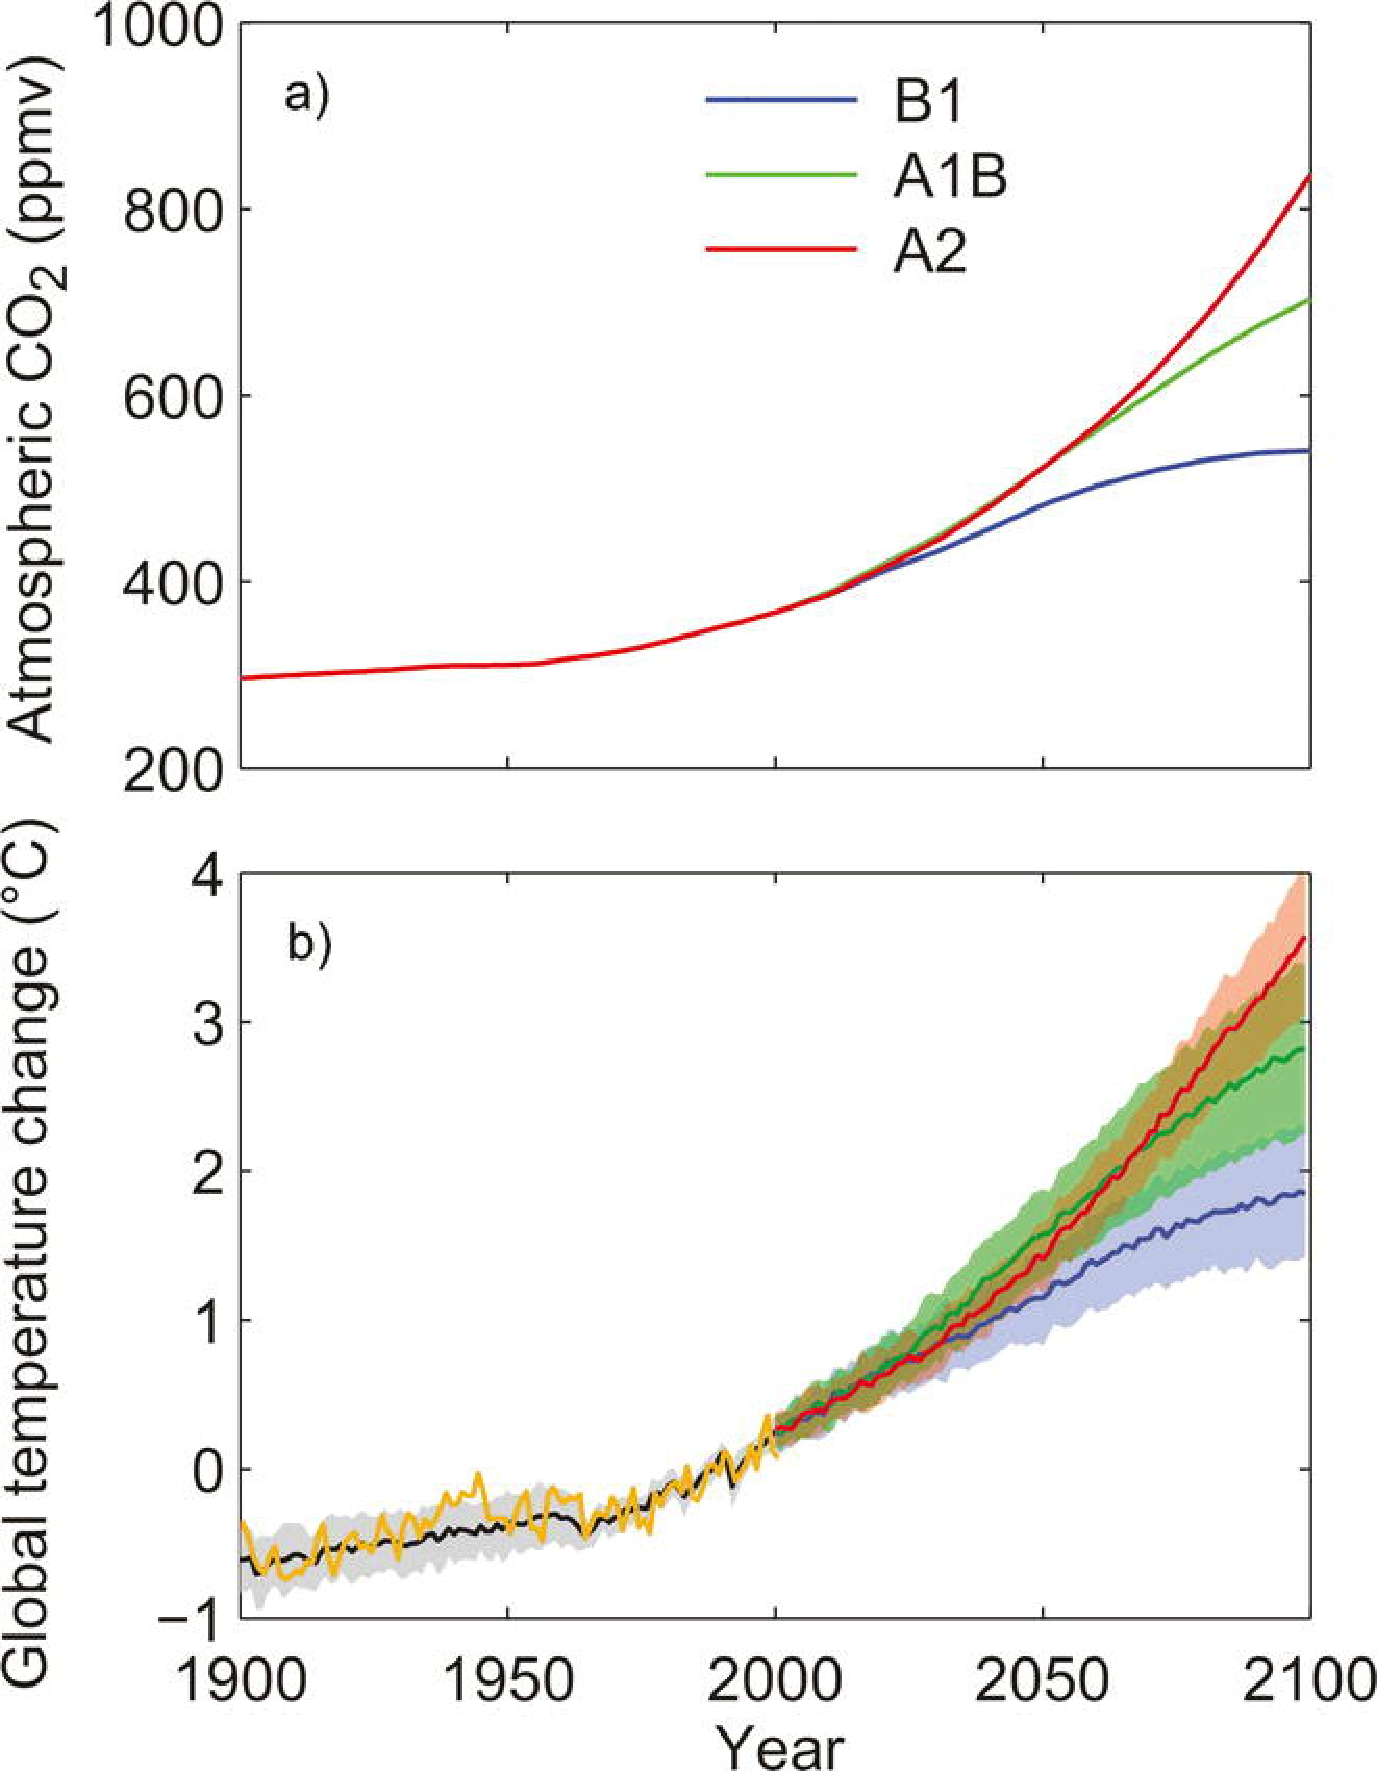
\includegraphics[width=19pc]{figure01.pdf}}
  \caption{Enter the caption for your figure here.  Repeat as
  necessary for each of your figures. Figure from \protect\cite{Knutti2008}.}\label{f1}
\end{figure}

\begin{figure}
\centerline{(illustration here)}
\appendcaption{A1}{Here is the appendix figure caption.}
\end{figure}

\begin{figure}
\centerline{(illustration here)}
\appendcaption{B1}{Here is the appendix figure caption.}
\end{figure}



\end{document}
%%%%%%%%%%%%%%%%%%%%%%%%%%%%%%%%%%%%%%%%%%%%%%%%%%%%%%%%%%%%%%%%%%%%%
% END OF AMSPAPER.TEX
%%%%%%%%%%%%%%%%%%%%%%%%%%%%%%%%%%%%%%%%%%%%%%%%%%%%%%%%%%%%%%%%%%%%%